\section{Theorie}
\label{sec:Theorie}
Theoretische Grundlagen für dieses Experiment sind das Biot--Savartsche Gesetz, der Hall-Effekt, elektromagnetsiche Induktion und Ferromagnetismus.
%so, ich hoffe ich vergesse nicht, dir eine Sprachnachricht zu schicken, dass ich das hier sehr kleinlch gemacht habe. auch, weil ich deine Notizen im letzten Versuch z.großenT. sehr hilfreich gefunden habe

Magnetfelder bilden sich durch bewegte Ladungen, wie beispielsweise durch elektrischen Strom. %im ersten Moment fragte ich mich zwar "durch was sonst", aber klar Spins und Umlaufbahnen um Protonen. habe aber das Wort "elektrischen" hinzugefügt
Eine Quantifizierung der Feldstärke $\symbf{H}$ wird durch das Biot--Savart-Gesetz 
\begin{equation}
\symbf{H}=\frac{I}{4\symup{\pi}}\int_\Gamma \frac{\symup{d}\symbf{s}\times\symbf{r}}{r^3} %da PI konstant, müsste es nicht symup sein? *thinking emoji* <- der fehlt mir irgendwie, um solchen Fragen den Vorwurfcharakter zu nehmen
\label{eqn:biotsavart}
\end{equation}
gegeben, bei dem über 
%die Leiterschleife | muss ja nicht zwingend eine Schleife, bzw. ein geschlossener Weg sein
den Leiter $\Gamma$ integriert wird. % oder einfach Leiterverlauf, oder Leiterweg.. kp. man sollte ja eigentlich wissen, dass Gamma ein linearer Verlauf ist
Für das Vakuum und Materialien, deren magnetische Momente aufgrund der Wärmebewegung statistisch verteilt sind, gilt der %'das' Vakuum, da Einzahl und bestimmt
Zusammenhang 
\begin{equation}
\symbf{B}=\symup{\mu_0}\mu_r\symbf{H}
\end{equation}
für die magnetische Flussdichte $\symbf{B}$. 
Dabei sind $\symup{\mu_0}=4\symup{\pi} \cdot 10^{(-7)} \, \si{\volt\second\ampere\tothe{-1}\meter\tothe{-1}}$ die Permeabilitätskonstante 
und $\mu_r$ die materialabhängige, relative Permeabilität. %Kommasetzung bei Adjektiven, die sich auf dasselbe Nomen beziehen. Ansonsten bezöge sich das erste auf das zweite Adjektiv und wäre damit ein Adverb

Die Untersuchung des Stoffmagnetismus, wie sie in diesem Versuch unter anderem vorgenommen wird, erfordert die Unterteilung 
in Para-, Dia- und Ferromagneten. 
Die relative Permeabilität $\mu_r$ von sowohl Para-, als auch Diamagneten ist eine konstante Zahl. 
Das bedeutet 
%im Umkehrschluss | ich glaube ein Umkehrschluss würde sich in diesem Kontext auf den Ferromagneten beziehen. Ich würde sagen, es 'folgt' einfach aus der Konstanz
, dass sich das im Material durch die Stoffeigenschaften zusätzlich ausbildende Magnetfeld, die 
sogenannte Magnetisierung 
\begin{equation}
\symbf{M}=\frac{1}{\symup{\mu_0}}\symbf{B}_\text{Materie}-\symbf{H}_\text{Vakuum}=\symbf{H}_\text{Vakuum}(\symup{\mu_0}-1) \text{,} 
\label{eqn:Magnetisierung}
\end{equation}
parallel zum äußeren Feld $\symbf{H}$ ist. 
Beim Diamagneten ist die Parallelität vielmehr eine Antiparallelität; das heißt, $\symbf{M}$ hat eine das Feld
abschwächende Wirkung und der Magnet wird aus Bereichen hoher Feldstärke herausgestoßen. 
Daraus ergibt sich, dass $\symup{\mu_0}-1 < 0$, also $\symup{\mu_0}<1$ gelten muss. 

Genau entgegengesetzt ist es beim Paramagneten: Hier gilt echte Parallelität, also $\symup{\mu_0}-1 > 0$ beziehungsweise 
$\symup{\mu_0}> 1$, der Magnet hat eine das Feld verstärkende Wirkung und wird in Gebiete hoher Feldstärke hineingezogen.

Ferromagneten 
%legen ein anderes Verhalten an den Tag | ich glaube es ist ein wenig umgangsprachlich (und vllt. nicht wissenschaftlich), Metaphern zu verwenden :P
hingegen verhalten sich deutlich anders
: Die relative Permeabilität ist keine Konstante, sondern vielmehr 
eine komplizierte Funktion des angelegten Feldes $\symbf{H}_\text{Vakuum}$, die %von der Geschichte des Materials abhängt.
davon abhängt, in welchen Zuständen das Material welcher Magnetfeldstärke ausgesetzt war, und ist damit \textit{zustandsabhängig}. %zwar ist hier zweimal das Wort Zustand, aber es folgt ja das Adjektiv aus der vorigen Erklärung. ich glaube dann passt das
Anhand einer Hysteresekurve, bei der die Magnetisierung $\symbf{M}$ auf das äußere Magnetfeld $\symbf{H}_\text{Vakuum}$ 
aufgetragen wird, wird das Verhalten solcher Magneten im Folgenden erklärt. 
%HIER NOCH BILD VON HYSTERESE EINFÜGEN
\FloatBarrier
\begin{figure}
    \centering
    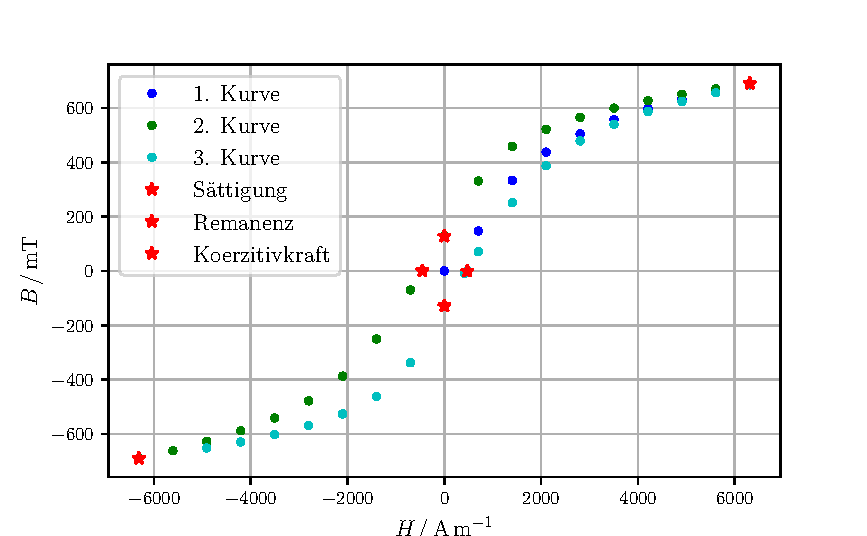
\includegraphics{plot_Hysterese.pdf}
    \caption{Hysteresekurve eines Ferromagneten.}
    \label{fig:hysterese}
\end{figure}
\FloatBarrier

Ferromagneten besitzen sogenannte \textit{Weiß'sche Bezirke}, in denen die Teilchen das gleiche magnetische Dipolmoment besitzen. 
Ist der Magnet unmagnetisiert, ist deren Ausrichtung statistisch verteilt und sie kompensieren sich, sodass $\symbf{M}=0$ gilt. %statistisch verteit klingt echt cool. aber kann man dazu angeben, welche Art von Verteilung oder versteht man darunter einfach schon eine gleichmäßige Verteilung? *te*
Wird nun ein äußeres Magnetfeld $\symbf{H}_\text{Vakuum}$ angelegt, richten sich bei steigender Magnetfeldstärke immer mehr Weiß'sche Bezirke entlang des 
Feldes aus, wodurch sich diese vergrößern. 
Dies geschieht bis zu einer Obergrenze; die \textit{Sättigung} des Materials wird erreicht. 
Wird nun %$\symbf{H}_\text{Vakuum}$ wieder verringert und ganz abgeschaltet
das äußere Magnetfeld wieder entfernt, bleibt eine Restmagnetisierung übrig, 
die sogenannte \textit{Remanenz}. 
Erst bei Anlegen eines entgegengesetzten Magnetfeldes verschwindet die Magnetisierung. 
Die dafür notwendige Feldstärke ist die \textit{Koerzitivfeldstärke}. %kann man auch Erregung schreiben? *te*
Dasselbe kann nun in die andere Richtung durchlaufen werden: $\symbf{H}_\text{Vakuum}$ wird im Negativen 
maximiert, bis der Ferromagnet in entgegensetzter Richtung seine magnetisische Sättigung erreicht, danach wieder 
bis ins Positive gesteigert, sodass der Magnet die Punkte der Remanenz und Koerzitivfeldstärke mit anderem Vorzeichen 
durchläuft. 

Die Magnetfelder werden mit einer Hall-Sonde gemessen, die auf folgender Funktionsweise beruht:
Die stromdurchflossene Messspitze wird in das entsprechende Magnetfeld gehalten.
Da Magnetfelder auf bewegte Ladungen die Lorentzkraft $F_L$ ausüben, werden %die Ladungsträger alle | ugs.
alle Ladungsträger in die gleiche Richtung
abgelenkt. Dies passiert solange, bis sich die Lorentzkraft mit %der elektrischen Kraft kompensiert, die | Bestimmte-Artikel-Schlacht xD
%jener elektrischen Kraft kompensiert, welche | nicht sicher tho ob das besser ist
%sich gleichnamige Ladungen abstoßen lässt. 
% hier fällt mir gerade auf. wir kennen ja "jene Kraft".. muss man dann ja nicht so umschreiben
der Coulombkraft für gleiche Ladungen kompensiert.
Es hat sich eine stabile Ladungskonfiguration ausgebildet, zwischen der sich die \textit{Hall-Spannung} 
messen lässt. Daraus lässt sich dann das zu messende Magnetfeld berechnen. Die Hall-Sonde zeigt den %sich ergebenden Wert für
Wert als die magnetische Flussdichte $\symbf{B}$ an. 
Es gibt verschiedene Modelle von Sonden; transversale und longitudinale. Diese unterscheiden sich alleinig durch die 
Orientierung der Messspitze. Die Wahl des Modells hängt also nur von der Geometrie der Messung ab. %und hat keiner tiefergehende Bedeutung.

Ergänzend zu dem Biot--Savart'schen Gesetz seien hier noch einige Magnetfeldinstallationen vorgestellt, die für das Experiment %du hast oben mein Bindestrich korrigiert und hier einen einzelnen gemacht :P
von Bedeutung sind.

Mithilfe \eqref{eqn:biotsavart} ergibt sich für einen stromdurchflossenen Drahtring mit Radius $R$ auf seiner durch den Kreismittelpunkt 
gehenden Symmetrieachse (der Parameter $x$ sei im Kreismittelpunkt Null)
\begin{equation}
    \lvert\symbf{B}_\text{Ring}(x)\rvert = B_\text{Ring}(x) = \frac{\symup{\mu_0 I}}{2} \frac{R^2}{(R^2 + x^2)^{\frac{3}{2}}}.
    \label{eqn:ring}
\end{equation}
Werden zwei Drahtringe bei $x=\sfrac{d}{2}$ und $x=\sfrac{-d}{2}$ positioniert und in gleicher Richtung mit Strom durchflossen,
gilt gemäß des Superpositionsprinzips: 
\begin{equation}
    B_d(x)=B_\text{Ring}(x-\frac{d}{2}) + B_\text{Ring}(x+\frac{d}{2})
    \label{eqn:2ringe}
\end{equation}

Das B-Feld innerhalb einer langen Spule ist nahezu homogen, sofern die Länge $l$ sehr viel größer als der Radius $R$ ist. 
Die Magnetfeldlinien innerhalb verlaufen parallel zur Symmetrieachse und bilden außerhalb einen großen 
Bogen vom Ende zum Anfang der Spule, sodass geschlossene Feldlinien durch die Spule laufen.
Innerhalb der Spule gilt abgesehen von Randeffekten 
\begin{equation}
    B_\text{Sp} = \mu_r \symup{\mu_0} \frac{n}{l} I
    \label{eqn:langespule}
\end{equation}
für die Flussdichte mit der Windungszahl $n$ und dem Strom $I$. 
Wird die lange Spule zu einem Kreis gebogen, entsteht eine Toroidspule, außerhalb der das Magnetfeld Null ist und bei der 
die Randeffekte verschwinden. 
Für die Flussdichte gilt mit \eqref{eqn:langespule} und durch Ersetzung der Länge $l$ durch den Umfang des Toroiden des Radius $r_T$:
\begin{equation}
    B_T=\mu_r \symup{\mu_0} \frac{n}{2 \symup{\pi} r_T} I
    \label{eqn:toroid}
\end{equation}
